\documentclass[11pt]{beamer}
\usepackage[utf8]{inputenc}
\usepackage[T1]{fontenc}
\usepackage{lmodern}
\usepackage[french]{babel}
\usetheme{Antibes}
\usepackage{subfig}
\usepackage{algorithm}
\usepackage{algorithmic}
%%% Packages additionnels
\usepackage{verbatim}
\usepackage{bbm}
\usepackage{stmaryrd}
\usepackage[numbered,framed]{matlab-prettifier}
\usepackage{listings}

\renewcommand{\algorithmicrequire}{\textbf{Entrée(s) :}}
\renewcommand{\algorithmicreturn}{\textbf{retourner}}
\renewcommand{\algorithmicensure}{\textbf{Initialisation ;}}
\renewcommand{\algorithmicwhile}{\textbf{Tant que}}
\renewcommand{\algorithmicdo}{\textbf{Initialisation}}
\renewcommand{\algorithmicendwhile}{\textbf{fin du Tant que ;}}
\renewcommand{\algorithmicend}{\textbf{fin}}
\renewcommand{\algorithmicif}{\textbf{si}}
\renewcommand{\algorithmicendif}{\textbf{fin du si}}
\renewcommand{\algorithmicelse}{\textbf{sinon}}
\renewcommand{\algorithmicelsif}{\textbf{fin du sinon}}
\renewcommand{\algorithmicthen}{\textbf{alors}}
\renewcommand{\algorithmicthen}{\textbf{Étape E}}
\renewcommand{\algorithmicthen}{\textbf{Étape M}}
\renewcommand{\algorithmicfor}{\textbf{pour}}
\renewcommand{\algorithmicforall}{\textbf{pour tout}}
\renewcommand{\algorithmicto}{\textbf{à}}
\renewcommand{\algorithmicendfor}{\textbf{fin du pour}}
\renewcommand{\algorithmicdo}{\textbf{faire}}
\renewcommand{\algorithmicloop}{\textbf{boucler}}
\renewcommand{\algorithmicendloop}{\textbf{fin de la boucle}}
\renewcommand{\algorithmicrepeat}{\textbf{répéter}}
\renewcommand{\algorithmicuntil}{\textbf{jusqu’à}}

\setbeamertemplate{blocks}[rounded][shadow=true]
\makeatother
\setbeamertemplate{footline}
{
	\leavevmode%
	\hbox{%
		\begin{beamercolorbox}[wd=.33\paperwidth,ht=2.25ex,dp=1ex,center]{author in head/foot}%
			\usebeamerfont{author in head/foot}\insertshortauthor
		\end{beamercolorbox}%
		\begin{beamercolorbox}[wd=.33\paperwidth,ht=2.25ex,dp=1ex,center]{title in head/foot}%
			\usebeamerfont{title in head/foot}\insertshorttitle
		\end{beamercolorbox}%
		\begin{beamercolorbox}[wd=.33\paperwidth,ht=2.25ex,dp=1ex,center]{date in head/foot}%
			\usebeamerfont{date in head/foot}\insertshortdate\hspace*{3em}
			\insertframenumber{} / \inserttotalframenumber\hspace*{1ex}
	\end{beamercolorbox}}%
	\vskip0pt%
}
\makeatletter
\setbeamertemplate{itemize item}[ball]
\setbeamertemplate{itemize subitem}[triangle]
\setbeamertemplate{itemize subsubitem}[circle]



\AtBeginSection[]{\begin{frame} \tableofcontents[currentsection] \end{frame}}


\begin{document}
	\author{CARVAILLO, CÔME, PRALON}
	\title[Projet UE HAX817X]{Un modèle pour les nids d'oiseaux}
	\subtitle{}
	\logo{
		\begin{minipage}[c]{1.15\linewidth}
			
\includegraphics[height=0.6cm]{logo.png} \hspace{0.65truecm}\hfill 
			
\includegraphics[height=0.6cm]{imag_logo.png}
			\hspace{0.65truecm}\hfill 
			
\includegraphics[height=0.6cm]{fds_logo.png}
		\end{minipage}
	}
	\institute[Université de Montpellier]{Soutenance de projet de Master 1}
	\date{3 juin 2022}
	%\subject{}
	%\setbeamercovered{transparent}
	\setbeamertemplate{navigation symbols}{}
	%	\begin{frame}[plain]
		%		\maketitle
		%	\end{frame}
	\frame{\titlepage}
	%	\begin{frame}
		%		\frametitle{}
		%	\end{frame}
	
	%%%%%%%%%%%%%%%%%%%%%%%
	\section{Introduction}
	
	
	\section{Liminaires théoriques et modélisation du problème}
	
	\begin{frame}{Définition et hypothèses}
		\begin{block}{Loi de mélange}
			Si l'on se donne $J$  densités $f_1(x), \cdots, f_J(x)$, alors toute variable aléatoire $X$ dont la densité $f$ s'exprime, pour tout $x\in\mathbbm{R}$, sous la forme
			\[
			f(x) := \displaystyle\sum_{j=1}^J \alpha_j f_j(x)
			\]
			où
			\[
			\alpha_j \in\mathbbm{R}_+^* \text{ et } \displaystyle\sum_{j=1}^J\alpha_j=1
			\]
			suit une loi de mélange continue.
		\end{block}
	\end{frame}
	

	\begin{frame}{Définitions et hypothèses}
		\begin{block}{Vecteurs des paramètres}
			\[
			\theta = (\alpha_j, \mu_j, v_j)_{j \in \llbracket 1,J\rrbracket}
			\]
		\end{block}
		
		\begin{block}{Une histoire de variables}
			Nous introduisons les deux variables aléatoires (V.A.) suivantes :
			\begin{itemize}
				\item la V.A. $X$, modélisant le volume des nids, de densité $f$
				\item la V.A. discrète $Z \in \llbracket 1,J\rrbracket$, représentant l'espèce d'oiseau
			\end{itemize}
		\end{block}


	\end{frame}


	\begin{frame}{Définitions et hypothèses}
		\begin{block}{Hypothèse 1}
			$X$ conditionnellement à $(Z = j)$ est une loi normale $\mathcal{N}(\mu_j, v_j)$
		\end{block}
		\begin{block}{Hypothèse 2 (Existence)}
			Soit \[
			\Theta := \{ \theta = (\alpha_j,\mu_j, v_j)_{1 \leq j \leq J} \text{ } \big| \text{ } \alpha_j > 0 \text{ } \forall j\in \llbracket 1,J\rrbracket \text{ et } \displaystyle\sum_{j=1}^J\alpha_j=1\}
				 \]
Soit $X_1, \cdots, X_n$ un échantillon de même loi que $X$. \newline
On supposera qu'il existe un $\theta \in \Theta$ tel que les données récoltées soient la réalisation du précédent échantillon.
		\end{block}
	\end{frame}

	\begin{frame}{Une histoire de densités}
		\begin{block}{Diverses densités}
			\begin{itemize}
				\item Densité de la loi $X$ conditionnellement à $(Z=j)$ :
				\[
				f(x| Z = j)  = \gamma_{\mu_j, v_j}(x)
				\]
				\item Densité de la loi de $X$ :
					\[
					f_\theta(x) = \displaystyle\sum_{j=1}^J \alpha_j \gamma_{\mu_j, v_j}(x)
					\]
				\item Probabilité de la loi de $Z$ conditionnellement à $(X = x)$ : 
					\[
					\mathbbm{P}_\theta(Z = j | X = x)=\displaystyle \frac{\gamma_{\mu_j, v_j}\times\alpha_j}{f_\theta(x)}
					\]
			\end{itemize}
		\end{block}
	\end{frame}

	

	\begin{frame}{Une approche idéaliste}
		\begin{block}{Le modèle}
			\begin{itemize}
				\item Nous observons et le volume et l'espèce d'oiseau
				\item Log-vraisemblance du modèle :
				\begin{align*}
				& \mathcal{L}_\theta(X_1, \cdots, X_n, Z_1, \cdots, Z_n) \\
				&=\displaystyle\sum_{j=1}^J \#A_j ln(\alpha_j)+ \sum_{j=1}^J\sum_{i\in A_j} ln(\gamma_{\mu_j, v_j}(X_i))
				\end{align*}
				où
				\[
				A_j := \{ i\in \llbracket1,n \rrbracket \text{ tels que } Z_i = j \}
				\]
			\end{itemize}
		\end{block}
	\end{frame}

	\begin{frame}{Une approche idéaliste}
		\begin{block}{Estimateurs du maximum de vraisemblance (EMV)}
			\[
			\widehat{\alpha_j} = \frac{\#A_j}{n}
			\]
			\[
			\widehat{\mu_j} = \displaystyle\frac{\sum_{i\in A_j} X_i}{\#A_j}
			\]
			\[
			\widehat{v_j} = \displaystyle \frac{\sum_{i\in A_j}(X_i - \widehat{\mu_j})^2}{\#A_j}
			\]
		\end{block}
	\end{frame}


	\begin{frame}{Une approche réaliste}
		\begin{block}{Le modèle}
			\begin{itemize}
				\item Nous observons seulement le volume des nids
				\item Log-vraisemblance du modèle :
				\begin{align*}
					& \mathcal{L}_{obs}(\theta, X_1, \cdots, X_n) \\
					&= ln\left( \displaystyle\prod_{i=1}^n f_\theta(X_i) \right)\\
					&= \displaystyle\sum_{i=1}^nln\left( \sum_{j=1}^J \alpha_j \gamma_{\mu_j, v_j}(X_i) \right)
				\end{align*}
			\end{itemize}
		\end{block}
	\end{frame}


	\begin{frame}{Log-vraisemblance conditionnelle}
		\begin{block}{Problème et solution}
			\begin{itemize}
				\item L'existence d'une expression analytique des EMV n'est pas assurée
				\item Nécessité de construire une méthode permettant d'approcher les valeurs des estimateurs

				\item Nous définissons ainsi la log-vraisemblance conditionnelle comme :
					\[
					\mathcal{L}_{c}(\theta, \tilde{\theta}, X_1, \cdots, X_n)
					\]
					\[ = \mathbbm{E}_{\tilde{\theta}}[\mathcal{L}_\theta(X_1, \cdots, X_n, Z_1, \cdots, Z_n) | X_1, \cdots, X_n]
					\]

			\end{itemize}
		\end{block}
	\end{frame}


	\begin{frame}{Réécritures}
		\begin{block}{Log-vraisemblance conditionnelle}
			\scriptsize
			\begin{itemize}
				\item Première forme :
				\[
				\mathcal{L}_{c}(\theta, \tilde{\theta}, X_1, \cdots, X_n) = \displaystyle\sum_{i=1}^n\sum_{j=1}^J ln(h_\theta(X_i ,j))  \mathbbm{P}_{\tilde{\theta}}(Z = j|X = X_i)
				\]
				\item Seconde forme :
				\begin{align*}
				 & \mathcal{L}_{c}(\theta, \tilde{\theta}, X_1, \cdots, X_n) \\
				 &= -\frac{n}{2}ln(2\pi)+\sum_{j=1}^J \left(\sum_{i = 1}^n \mathbbm{P}_{\tilde{\theta}}(Z= j|X=X_i)\right) \times ln(\alpha_j) \\				
				&-\frac{1}{2}\sum_{j=1}^J\left(\sum_{i=1}^n  \mathbbm{P}_{\tilde{\theta}}(Z=j|X=X_i)\times\left(log(v_j)+\frac{(X_i-\mu_j)^2}{v_j}\right)\right)
				\end{align*}

			\end{itemize}
		\end{block}
	\end{frame}

	\begin{frame}{Log-vraisemblance conditionnelle}
		\begin{block}{Estimateurs du maximums de vraisemblance}
			\[
			\widehat{\alpha_j} = \displaystyle\frac{1}{n}\sum_{i=1}^n \mathbbm{P}_{\tilde{\theta}}(Z=j|X=X_i)
			\]
			\[
			\widehat{\mu_j}= \displaystyle\frac{\displaystyle\sum_{i=1}^n X_i\times\mathbbm{P}_{\tilde{\theta}}(Z=j|X=X_i)}{\displaystyle\sum_{i=1}^n \mathbbm{P}_{\tilde{\theta}}(Z=j|X=X_i)}
			\]
			\[
			\widehat{v_j} = \displaystyle\frac{\displaystyle\sum_{i=1}^n (X_i -\widehat{\mu_j})^2 \times\mathbbm{P}_{\tilde{\theta}}(Z=j|X=X_i)}{\displaystyle\sum_{i=1}^n\mathbbm{P}_{\tilde{\theta}}(Z=j|X=X_i)}
			\]			
		\end{block}
	\end{frame}
	

	\section{L'algorithme EM}
	\begin{frame}{L'algorithme EM}
		\begin{block}{\scriptsize But de l'implémentation de la fonction $algo\_EM$}
			\begin{itemize}
				\scriptsize
				\item Estimer les paramètres $\alpha_J$, $\mu_J$ et $\sigma_J$ du mélange gaussien
				\begin{itemize}
					\scriptsize
					\item $J$ est le nombre de gaussiennes présentent dans le mélange
				\end{itemize}
			\end{itemize}
		\end{block}
		\begin{block}{ \scriptsize Ses arguments}
			\begin{itemize}
				\scriptsize
				\item \textbf{\textit{data\_init}:} dataframe contenant les paramètres ($\alpha_{init}$, $\mu_{init}$, $\sigma_{init}$) initiaux choisis \\
				\item \textbf{\textit{X}:} Vecteur jouant le rôle de l'échantillon du mélange gaussien  \\
				\item \textbf{\textit{K}:} le nombre d'itérations de l'algorithme EM
			\end{itemize}
		\end{block}
		\begin{block}{\scriptsize Ce qu'elle retourne}
			\scriptsize
			\begin{itemize}
				\item Retourne un dataframe contenant les valeurs des paramètres $\widehat{\alpha_J}$, $\widehat{\mu_J}$ et $\widehat{\sigma_J}$ estimés par l'algorithme
			\end{itemize}
		\end{block}
	\end{frame}
	\begin{frame}{L'algorithme EM}
		\textbf{Pseudo code de l'algorithme EM, d'après [2]}
		\begin{figure}[H]
			\centering
			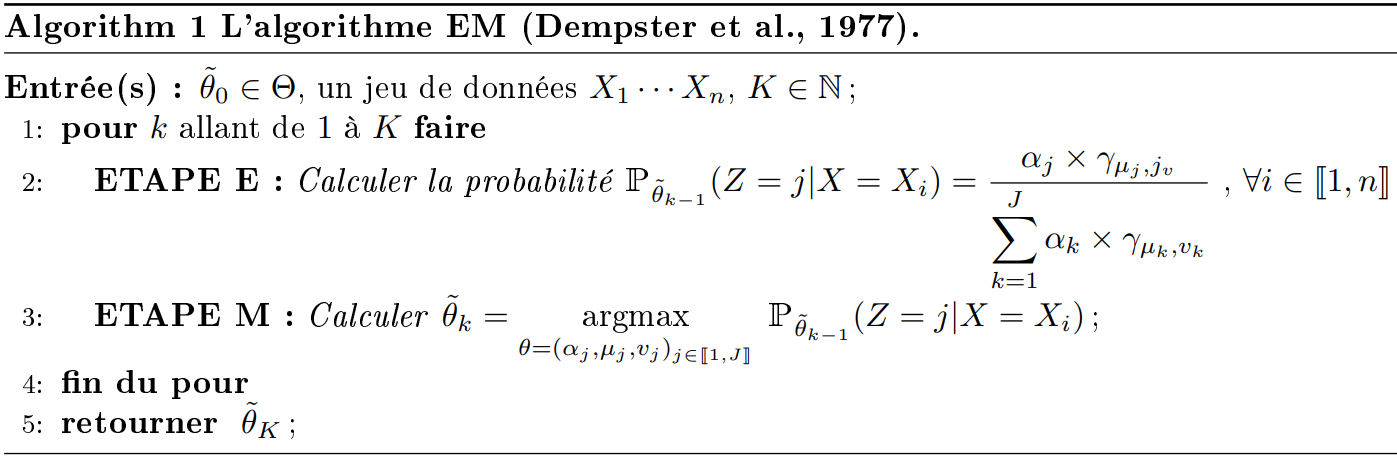
\includegraphics[scale=0.6]{images/pseudo_code.png}
		\end{figure}
	\end{frame}
	\begin{frame}{Les étapes de l'algorithme EM}
		\begin{block}{L'étape E (Expectation)}
			Consiste à déterminer $\mathbb{P}_{\tilde{\theta}}(Z = j | X = X_i)$ à l'aide de la formule suivante:
			\[
				\mathbb{P}_{\tilde{\theta}}(Z = j| X = X_i) = \frac{\alpha_j \times \gamma_{\mu_j, v_j}}{\sum_{k=1}^{J} \alpha_k \times \gamma_{\mu_k, v_k}}
			\]
		\end{block}
	\end{frame}
	\begin{frame}{Les étapes de l'algorithme EM}
		\begin{block}{L'étape M (Maximization)}
			Consiste à déterminer les EMV ($\widehat{\alpha_j}, \widehat{\mu_j}$, $\widehat{\sigma_j}$) de la log-vraisemblance conditionnelle via les formules suivantes:
			\begin{align*}
				\widehat{\alpha_j} &= \frac{1}{n}\sum_{i=1}^n \mathbb{P}_{\tilde{\theta}}(Z = j| X = X_i) \\
				\widehat{\mu_j} &= \frac{\sum_{i=1}^n X_i\mathbb{P}_{\tilde{\theta}}(Z = j| X = X_i)}{\sum_{i=1}^n \mathbb{P}_{\tilde{\theta}}(Z = j| X = X_i)} \\
				\widehat{v_j} &= \frac{\sum_{i=1}^n (X_i -\widehat{\mu_j})^2 \mathbb{P}_{\tilde{\theta}}(Z = j| X = X_i)}{\sum_{i=1}^n\mathbb{P}_{\tilde{\theta}}(Z = j| X = X_i)}
			\end{align*}
		\end{block}
	\end{frame}

	\begin{frame}{Un théorème de croissance}
		\begin{block}{Théorème}
			Soit $(\theta_k)_{k\in \llbracket1, K\rrbracket}$ la suite de paramètres construite à l'aide de l'algorithme EM. \newline
La log-vraisemblance $\mathcal{L}_{obs}$ des observations vérifie 
		\[
		\mathcal{L}_{obs}(\theta_{k+1}, X_1, \cdots, X_n) \geq \mathcal{L}_{obs}(\theta_k, X_1, \cdots, X_n)
		\]
		\end{block}
	\end{frame}

	\begin{frame}{Ersatz de preuve}
		\begin{block}{Démonstration: d'après [2] et [4]}
			\begin{itemize}
				\item Nous cherchons à montrer que
				\[
				\mathcal{L}_{obs}(\theta_{k+1}, X_1, \cdots, X_n) - \mathcal{L}_{obs}(\theta_k, X_1, \cdots, X_n) \geq 0 \text{   }(1)
				\]
				\item Réécriture :
				\[
				 \mathcal{L}_{obs}(\theta_{k+1}, X_1, \cdots, X_n) = 
				\mathcal{L}_c(\theta_{k+1}, \theta_k, X_1, \cdots, X_n) - \kappa_{\theta_{k+1},\theta_k}
				\]
				\item Avec
					\[
					 \kappa_{\theta_{k+1},\theta_k} = \sum_{i=1}^n\sum_{j=1}^J ln(\mathbbm{P}_{\theta_{k+1}}(Z = j|X=X_i))\times\mathbbm{P}_{\theta_k}(Z = j|X = X_i)
					\]
			\end{itemize}	
		\end{block}
	\end{frame}

	\begin{frame}{Ersatz de preuve}
		\scriptsize
		\begin{block}{Démonstration: d'après [2] et [4]}
				Ainsi,
				\[
				\mathcal{L}_{obs}(\theta_{k+1}, X_1, \cdots, X_n) - \mathcal{L}_{obs}(\theta_k, X_1, \cdots, X_n)
				\]
				\[
				= \underbrace{\mathcal{L}_c(\theta_{k+1}, \theta_k, X_1, \cdots, X_n) - \mathcal{L}_c(\theta_k, \theta_k, X_1, \cdots, X_n)}_{L} + \underbrace{\kappa_{\theta_{k}, \theta_k}  - \kappa_{\theta_{k+1}, \theta_k}}_{K}
				\]
Il s'agit de montrer 
				\[
			L + K \geq 0 \text{   } (2)
				\]
		\end{block}
	\end{frame}


	\begin{frame}{Ersatz de preuve}
		\begin{block}{Démonstration: d'après [2] et [4]}
			\begin{itemize}
				\item A l'étape M de l'algorithme, la quantité 
					\[
					\mathcal{L}_c(\theta, \theta_k, X_1, \cdots, X_n)
					\]
est maximisée en $\theta$, de maximum $\theta_{k+1}$
				\item Donc,
					\[
					\mathcal{L}_c(\theta_{k+1}, \theta_k, X_1, \cdots, X_n) - \mathcal{L}_c(\theta_k, \theta_k, X_1, \cdots, X_n) \geq 0
					\]
			\end{itemize}
		\end{block}
	\end{frame}

	\begin{frame}{Ersatz de preuve}
		\begin{block}{Démonstration: d'après [2] et [4]}
			\begin{itemize}
				\item Il reste donc à prouver que
					\[
					 K = \kappa_{\theta_{k}, \theta_k}, - \kappa_{\theta_{k+1}, \theta_k} \geq 0
					\]
				\item On montre que, après quelques fastidieux calculs,
				\begin{align*}
					& \kappa_{\theta_{k}, \theta_k}, - \kappa_{\theta_{k+1}, \theta_k} \\
					& \geq - n\times ln\left( \sum_{i=1}^n\sum_{j=1}^J\mathbbm{P}_{\theta_{k+1}}(Z = j|X=X_i)\times\frac{1}{n}\right)  \text{  }  (3) \\
					&=  -n\times ln(1)\\
					&= 0
				\end{align*}
			\end{itemize}
		\end{block}
	\end{frame}

	\begin{frame}
		\begin{block}{}
			\begin{itemize}
				\item Aucune preuve quant à la convergence de la suite $(\theta_k)_{k \in \llbracket 1, K \rrbracket}$ vers les EMV
				\begin{itemize}
					\item Stagnation dans des extremas locaux
				\end{itemize}
				\item Choix des paramètres initiaux crucial
			\end{itemize}
		\end{block}	
	\end{frame}

\section{La fonction \textit{Simulation}}
	
	\begin{frame}{La fonction \textit{Simulation}}
		\begin{block}{Son objectif}
			\small
			Générer aléatoirement un échantillon issu 
			d'un mélange gaussien
		\end{block}
		\begin{block}{Ses arguments}
			\begin{itemize}
				\small
				\item \textbf{\textit{Data\_th}:} le dataframe contenant les paramètres $\alpha_i$, $\mu_i$ et $\sigma_i$ où $i \in \{1, \dots ,J\}$ avec $J$ le nombre de mélanges gaussiens\\
				\item \textbf{\textit{n}:} Le nombre de valeurs que l'on souhaite générer aléatoirement
			\end{itemize}
		\end{block}
		\begin{block}{Ce qu'elle retourne}
			\begin{itemize}
				\small
				\item Un vecteur de taille $n$ généré aléatoirement
				\begin{itemize}
					\item Il s'agit de l'échantillon du mélange gaussien
				\end{itemize}
			\end{itemize}
		\end{block}
	\end{frame}
	\begin{frame}{Son principe de fonctionnement}
		\textbf{Exemple dans le cas d'un mélange à 3 gaussiennes}
		\begin{block}{Étapes répétées à chaques itérations}
			\begin{itemize}
				\item Génération d'une variable aléatoire $Z \sim \mathbb{U}(0,1)$
				\begin{itemize}
					\item Si $Z < \alpha_1$ alors $X \sim \mathcal{N}(\mu_1, \sigma_1)$ \\
					\item Sinon si $\alpha_1 \leq Z \leq \alpha_1 + \alpha_2$, alors $X \sim \mathcal{N}(\mu_2, \sigma_2)$ \\
					\item Sinon si  $\alpha_1 + \alpha_2 \leq Z \leq \alpha_1 + \alpha_2 + \alpha_3$, alors $X \sim \mathcal{N}(\mu_3, \sigma_3)$
				\end{itemize}
			\end{itemize}
		\end{block}
	\end{frame}
	

	\section{Études de simulations}


	\begin{frame}{Cas des variables à "fortes séparations" }
		\begin{figure}[htp] 
			\centering
			\subfloat[Boxplot des erreurs pour $\alpha_1$, $\alpha_2$ et $\alpha_3$]{%
				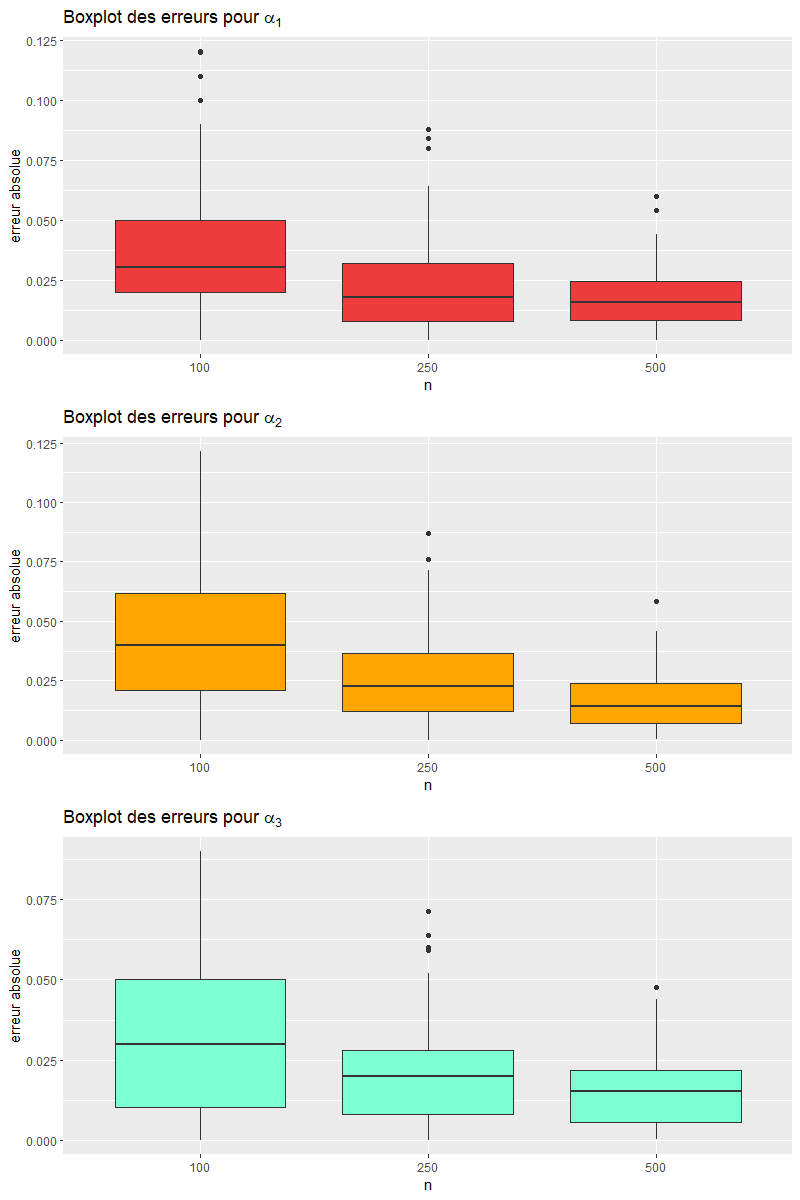
\includegraphics[scale=0.18]{images/good_alpha.png}%
			}%
			\hfill%
			\subfloat[Boxplot des erreurs pour $\mu_1$, $\mu_2$ et $\mu_3$]{%
				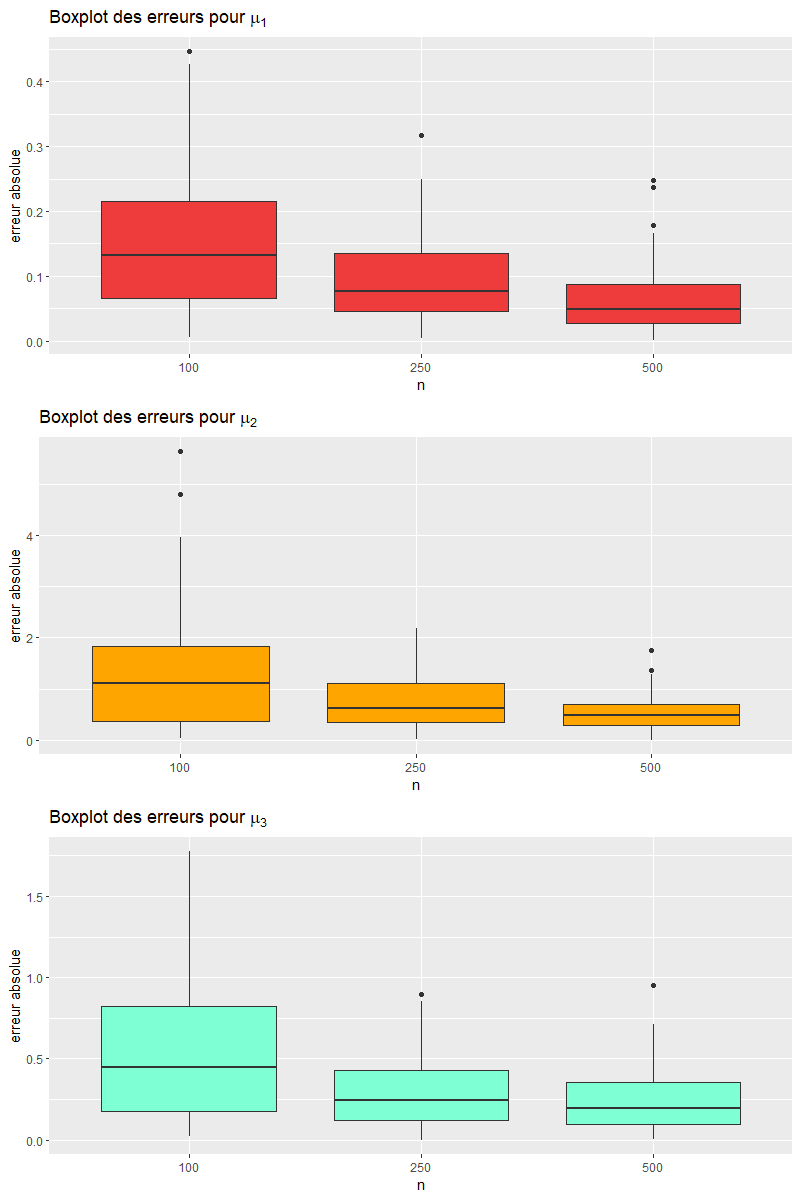
\includegraphics[scale=0.18]{images/good_mu.png}%
			}%
		\end{figure}
	\end{frame}

	\begin{frame}{Cas des variables à "faibles séparations" }
		\begin{figure}[htp] 
			\centering
			\subfloat[Boxplot des erreurs pour $\alpha_1$, $\alpha_2$ et $\alpha_3$]{%
				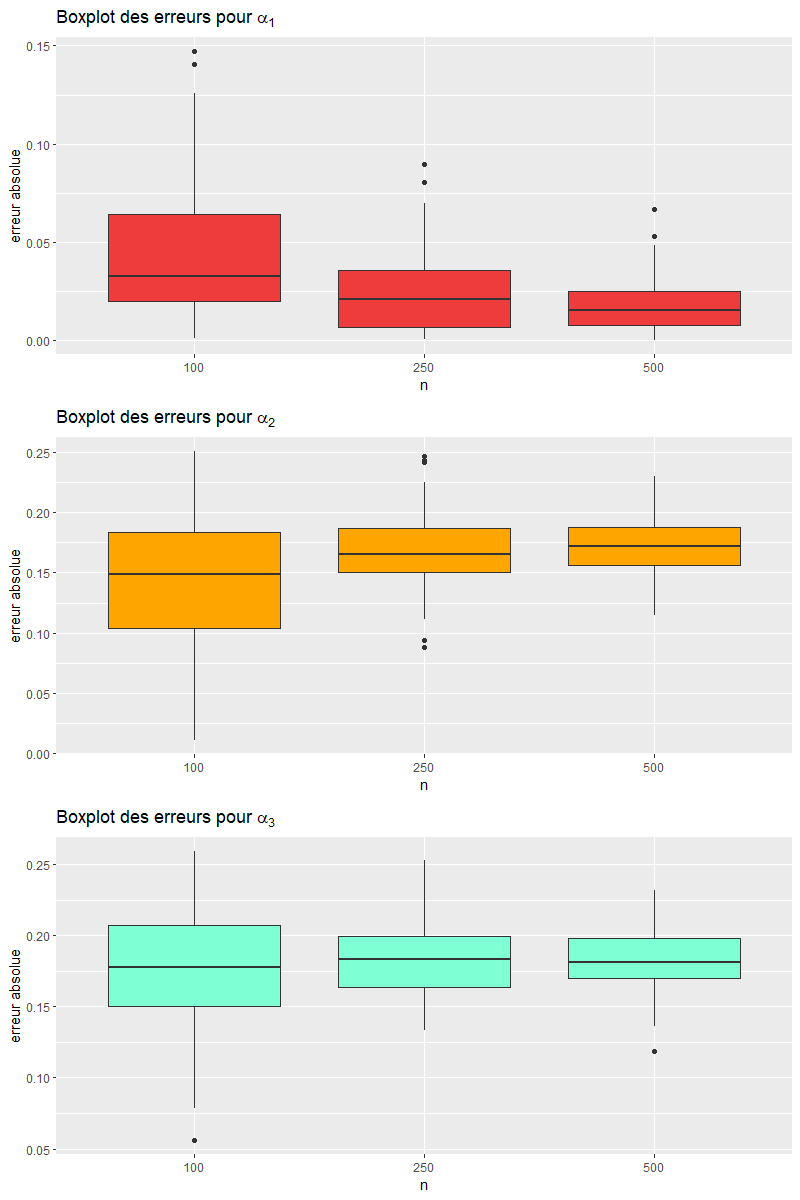
\includegraphics[scale=0.18]{images/bad_alpha.png}%
			}%
			\hfill%
			\subfloat[Boxplot des erreurs pour $\mu_1$, $\mu_2$ et $\mu_3$]{%
				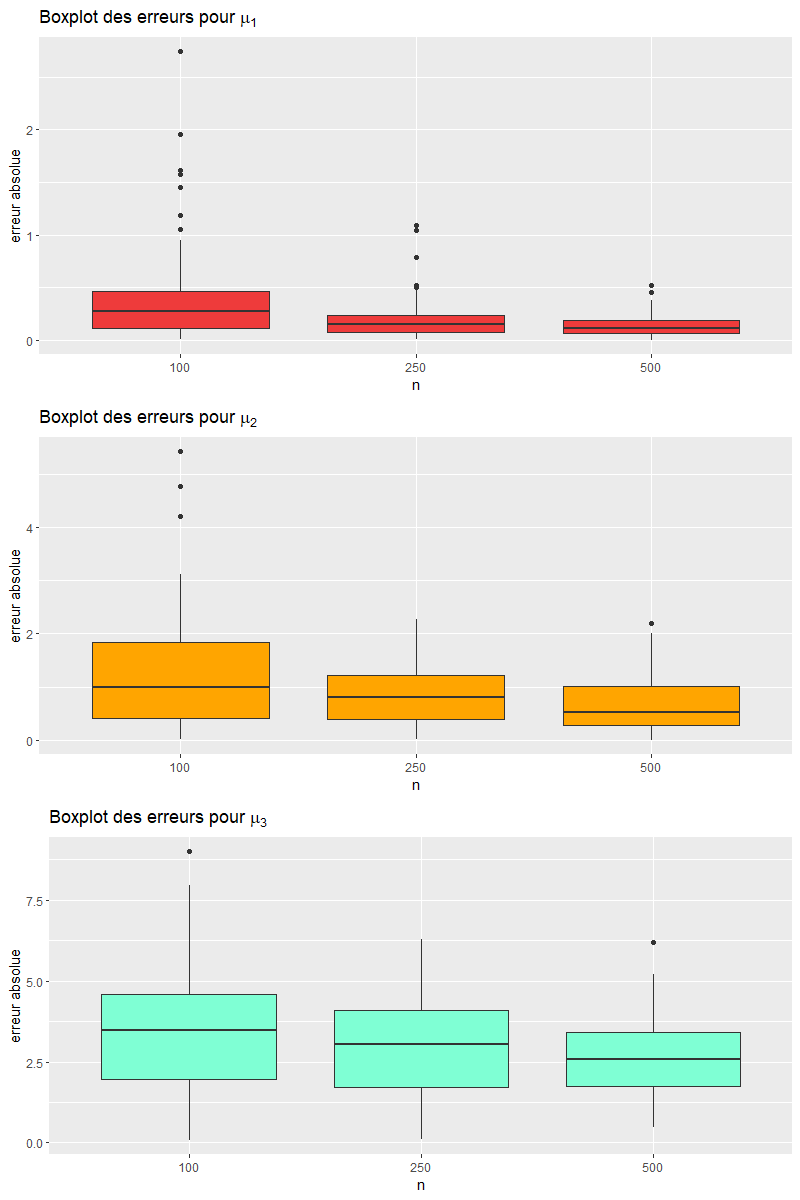
\includegraphics[scale=0.18]{images/bad_mu.png}%
			}%
		\end{figure}
	\end{frame}
	
	\section{Modélisation des nids d'oiseaux}

	\begin{frame}{Préambule}
		\begin{block}{Recueil des données}
			\begin{figure}[H]
				\centering
				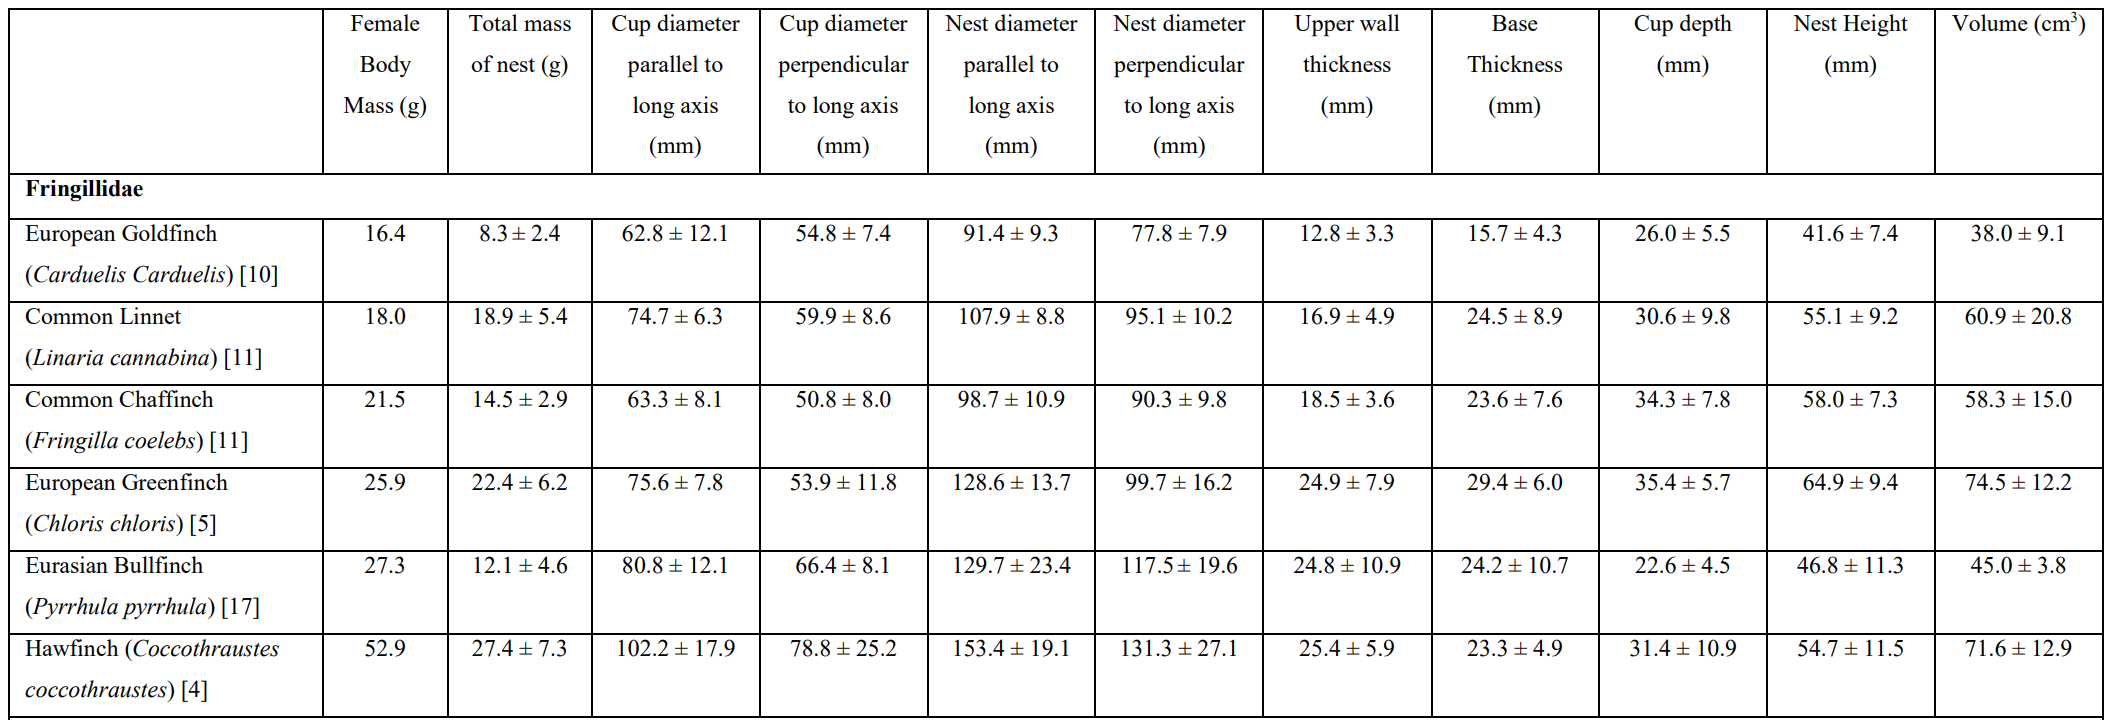
\includegraphics[scale=0.29]{tab_oiseaux.png}
				\caption{Caractéristiques des nids; d'après [5]}
			\end{figure}
		\end{block}
	\end{frame}	

	\begin{frame}{Hypothèses, outils et démarche}
		\begin{block}{\scriptsize Hypothèses}
			\begin{itemize}
				\scriptsize 
				\item la distribution du volume des nids d'une espèce donnée est gaussienne
				\item le nombre d'espèces $J$ est connu
			\end{itemize}
		\end{block}

		\begin{block}{\scriptsize Outils}
			\begin{itemize}
				\scriptsize 
				\item fonction \textit{simulation}
				\item fonction \textit{algo$\_$EM}
			\end{itemize}
		\end{block}

		\begin{block}{\scriptsize  Démarche}
			\begin{itemize}
				\scriptsize 
				\item Génération de l'échantillon
				\item Représentation graphique de la densité de l'échantillon
				\item Détermination des paramètres initiaux
				\item Execution de l'algorithme EM
			\end{itemize}
		\end{block}

	\end{frame}



	\begin{frame}{Première exploration des données}
		\begin{figure}[H]
			\centering
			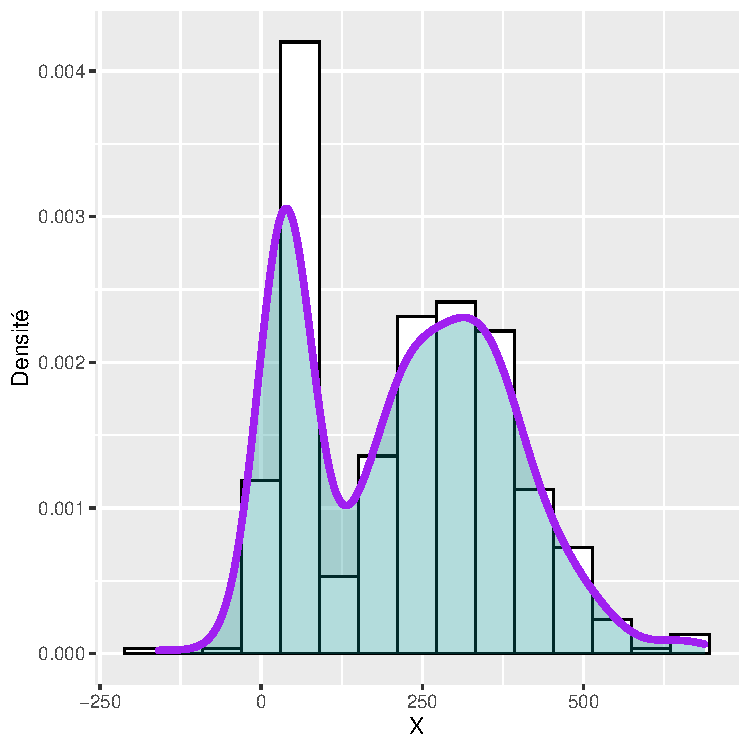
\includegraphics[scale=0.4]{dens1.pdf}
			\caption{Densité du mélange}
		\end{figure}
	\end{frame}

	\begin{frame}{Heuristique graphique}
		\begin{figure}[H]
			\centering
			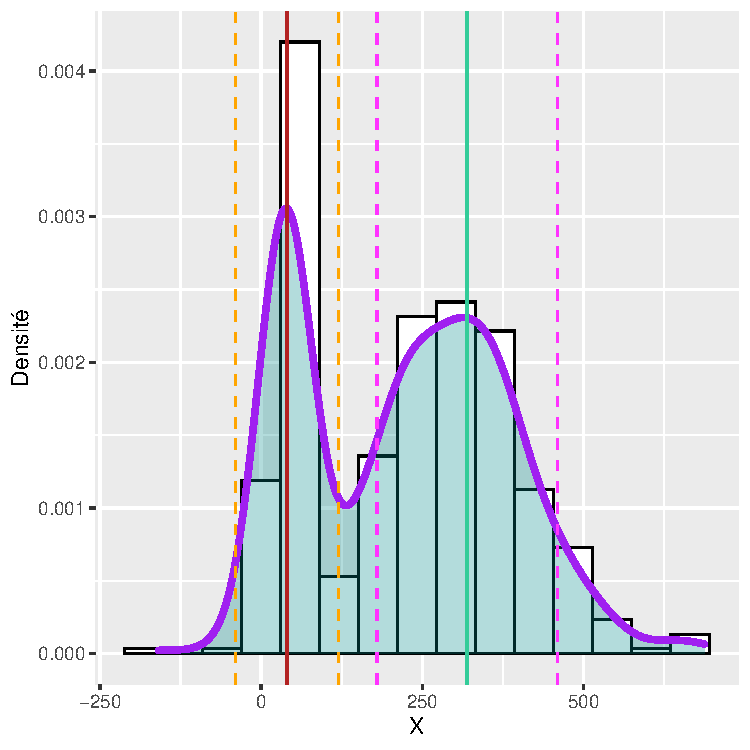
\includegraphics[scale=0.4]{dens1bis.pdf}
			\caption{Détermination des valeurs initiales}
		\end{figure}
	\end{frame}


	\begin{frame}[fragile]\frametitle{Heuristique graphique}
		\begin{block}{\scriptsize Paramètres initiaux}
			\begin{itemize}
				\scriptsize
				\centering
				\item $\mu_{1_{init}} =  40$ et $\mu_{2_{init}} = 320$
				\item $\sigma_{1_{init}} =  80$ et $\sigma_{2_{init}} = 140$
				\item $\alpha_{1_{init}} = 0.5$ et $\alpha_{2_{init}} = 0.5$
			\end{itemize}
		\end{block}
		\begin{block}{\scriptsize Résultats}
			\scriptsize
			\begin{verbatim}
          bird_names     alpha        mu      sigma
1 European Goldfinch 0.2910832  37.76285   9.512478
2         Ring Ouzel 0.7089168 302.51936 125.951894
			\end{verbatim}
		\end{block}
		\begin{block}{\scriptsize Valeurs théoriques}
			\scriptsize
			\begin{verbatim}
         bird_names2 proportion_alpha mean_volume sd_volume
1 European Goldfinch         0.2878713       38.0       9.1
12         Ring Ouzel        0.7121287      298.6     125.1
			\end{verbatim}
		\end{block}
	\end{frame}


	\begin{frame}{Détermination automatique}
		\begin{block}{}
			Comme dans le rapport ou fonction de Nicolas ??
		\end{block}
	\end{frame}


	\section{Conclusion}


	\section{Bibliographie}

	\begin{frame}
		\scriptsize
		\begin{enumerate}
		\item Dempster A.P., Laird N. M., Rubin D. B. (1977). Maximum Likelihood from Incomplete Data via the EM Algorithm, \textit{Journal of the Royal Statistical Society, Series B, Vol. 39, 1, 1-38}

		\item Chafai D., Malrieu F. (2018). Recueil de modèles aléatoires, 105-11, \textit{Prépublication}\newline
\url{https://hal.archives-ouvertes.fr/hal-01897577v3}

		\item Frédéric Santos (2015). L’algorithme EM : une courte présentation, \textit{Document de cours}
\newline\url{https://members.loria.fr/moberger/Enseignement/AVR/Exposes/algo-em.pdf} 

		\item Michael Collins (1997). The EM algorithm, \textit{Document de cours}\newline
\url{http://faculty.washington.edu/fxia/courses/LING572/EM_collins97.pdf} 

		\item Biddle L.E., Broughton R.E., Goodman A.M., Deeming D.C (2018). Composition of Bird Nests is a Species-Specific Characteristic, \textit{Avian Biology Research, Vol. 11, 2, 132-153}\newline
\url{https://core.ac.uk/download/pdf/155777956.pdf}
		\end{enumerate}
	\end{frame}


\end{document}